%%%%%%%%%%%%%%%% file mach.tex %%%%%%%%%%%%%%%%%
%                                                                                            %                                        
%          School of Computer Science & Engineering               %
%          The University of New South Wales                           %
%          Sydney, Australia                                                       %
%                                                                                            % 
%%%%%%%%%%%%%%%%%%%%%%%%%%%%%%%%%%%%%%%%%%%

\documentclass{sig-alternate}
\usepackage{multicol}
\begin{document}
%
% --- Author Metadata here ---
\conferenceinfo{Assignment 2} {June 5, 2011, Machine Learning, COMP9417}  
\CopyrightYear{2011}
%\crdata{978-1-59593-998-2/09/06}
% --- End of Author Metadata ---

\title{Using Reinforcement Learning for Traffic Lights Control}

\numberofauthors{3}
\author{
% 1st. author
\alignauthor
Han Li\\
       \email{hli@cse.unsw.edu.au}
       3299976
% 2nd. author
\alignauthor
Lawrence Yao\\
       \email{lawry@cse.unsw.edu.au}
       2252726
% 3rd. author
\alignauthor
Vaughan Rouesnel\\
       \email{vjro855@cse.unsw.edu.au}
       3188927
}

\subtitle{
    \textit{School of Computer Science and Engineering, The University of New South Wales, Sydney, Australia} \\
    \textit{COMP9417, Machine Learning, Assignment 3}
    }

\maketitle

\section {Introduction}

Reinforcement learning is naturally suited to control problems
since it readily fits the idea of agent and its environment and
in particular, learning on the job. Unlike classification algorithms,
it is not necessary to have a training set available. In this assignment,
we look at the problem of an agent controlling a traffic light with
three signals (red, amber, green) at a four roads (north-south,
south-north, east-west, and west-east) intersection. We implement various algorithms
and state representation, and compare their performance using
various parameters.


\section{Definition}

\subsection{Traffic Model}
The traffic is flowing in two ways on two intersecting roads. Based on the direction of car flows, the traffic model is comprised of four independent one-way flows, denoted as West-East, East-West, North-South and South-North. For example, in the North-South flow, all the cars travel in one direction, that is, from north to south.

The competing flows of the traffic are controlled by a set of traffic lights. As there are only two intersecting main roads (regardless the directions), two mutually exclusive traffic lights are sufficient. They are denoted as lightWE (which controls West-East and East-West), and lightNS, for North-South and South-North traffic flows. There are three signals, namely RED, AMBER and GREEN. A car should stop if there is an AMBER or RED signal, and the cars right behind it pile up in queue. In addition, the lights can not change consecutively in less than three timesteps.

Each flow is modelled as a standalone road. The road is 100 units in length (from 0 to 99), and intersects with the roads in the perpendicular directions at Unit 49 and 50. The traffic light is positioned at road intersections. At each timestep, one car enters the road at Position 0, with the probability that equals to the traffic intensity (e.g. 15\%). Cars are removed from the road when they reach the boundary (i.e., beyond Unit 99).

\subsection{State Representation}
The traffic state consists of the lights state and the cars state. As the light signals are mutually exclusive, there are only four possible states, namely (GREEN, RED), (AMBER, RED), (RED, GREEN) and (RED, AMBER), denoted as 0, 1, 2 and 3 respectively. Moreover, the value of light delay since last change is 0-3. Hence, the state space of lights is 4 x 4.

However, defining the cars state is less straightforward. The occupancy of each unit by a car can be marked as 0 or 1. As there are 48 units before the traffic lights on each road, the state space of cars can be as large as $2^{192}$. Therefore, we propose three variants of state representation to maintain the space in a feasible size.

\subsubsection{Default State}
The Default State is described in the assignment specification. On each road, only the position of the closest car from the intersection is counted, and only the first 9 units from the intersection are inspected. Therefore, the position is between 0 and 8 inclusive, and 9 denotes no cars. The space size of Default State is $10^4$.

\subsubsection{JamNess State}
The JamNess State is a representation of how busy the traffic is on that road (i.e. traffic jam-ness). Cars near the intersection weight heavier than cars far away from the intersection. To calculate JamNess, we introduce an importance value of each car, denoted as $0.5^i$, where $i$ is the position of the car from the traffic lights (at Unit 49). For example, the importance of the car at Unit 46 is $0.5^3$, since it is 3 positions away from the lights. The sum of all the importance values on one road is between 0 and 0.9999999. Then, the JamNess is calculated as $sum * 10$ and rounded down to an integer, which is between 0 and 9 inclusive. The space size of JamNess State is $10^4$.

\subsubsection{Occupancy State}
The Occupancy State represents the presence of cars at each unit. As discussed above, each unit is marked as 0 or 1, there are $2^{48}$ states if all the units are counted. However, since the traffic lights can be switched every three timesteps, we can speculate that the closest three or four positions from the intersection are more important than the rest. Hence, we define two states, Occ\_3 and Occ\_4, which are represented by a 3-bit and 4-bit integer respectively, indicating the occupancy of the closest three or four positions. For example, a binary value 100 in Occ\_3 indicates the first position is occupied, while the second and the third are empty. A binary value 0101 in Occ\_4 means the second and the fourth positions are occupied, whilst the rest are not. Since there are four roads, the space size of Occ\_3 is $2^{12}$, and that of Occ\_4 is $2^{16}$.

\subsubsection{Density State}
The Density State records the number of cars on the N closest positions from the intersection, where N is 3 in the implementation, since the traffic lights can only be switched every three timesteps. The number of cars in the closest three positions is between 0 and 3, so the space size of four roads is $4^4$ or $2^8$.

There is an extension of Density State (N=3). To help the controller predict the future traffic, we not only calculate the number of cars at the first three positions (i.e., from Unit 48 to 46), we also calculate the car number of the second three positions (i.e., from Unit 45 to 43). This extension is called Density\_6, as there are six positions involved. By constrast, Density State (N=3) is called Density\_3. The space size of this extension is $(4 * 4) ^{4}$, or $2^{16}$.

\section{Implementation}

\subsection{Learning Algorithms}

Reinforcement learning is concerned with how to learn a control policy (a mapping from the states of environment to control actions) so as to maximise a cumulative reward signal. Let $s_t$ be the state of the server at time $t$. The controller selects an action $a_t$ from a finite set $A$ resulting in the system transitioning to state $s_{t+1}$ at time $t+1$. The controller earns a reward $r_{t+1}$ for this transition. We implemented Sarsa, Q Learning and a OneRule algorithm as the benchmark.

\subsubsection{Sarsa}

This algorithm is based on the following formula from \cite{Sutton_1998} on page 145.

\begin{equation}
Q(s_{t},a_{t})\leftarrow Q(s_{t},a_{t}) + \alpha [ r_{t+1}+\gamma Q(s_{t+1},a_{t+1}) - Q(s_{t},a_{t}) ]
\end{equation}

where $\alpha $ is the learning rate, and $\gamma $ is the discount factor.

Some important implementation details are:

\begin{enumerate}
\item The 3 timesteps immediately
after a light switch is not involved in learning (i.e. $Q$ is not
updated in those 3 timesteps), however the reward is accumulated
during the 3 timesteps;

\item Sarsa uses the $\epsilon $-greedy policy, so
the best action is picked with probability $(1-\epsilon )$ and a
random action is picked with probability $\epsilon $. Picking
a random action means the light may switch with $50\%$ probability;

\item The $\epsilon $ is not discounted over time, although \cite{Sutton_1998}
mentions that Sarsa converges with probability 1 to an optimal policy
only if the policy converges in the limit to the greedy policy (which
requires $\epsilon $ to converge to 0 in the limit). The reason why
$\epsilon $ is not discounted is so it can be compared directly with
QLearningBasic algorithm using the benchmark settings.

\end{enumerate}

\subsubsection{Q Learning}

In Q-Learning~\cite{watkins_qlearning_1992}, the learning agent calculates the quality (or $Q$-value) of a state-action combination, denoted by $Q(s, a)$, from its interaction with the environment using the formula:
\begin{equation}
\begin{aligned}
Q_t(s_t, a_t) &= Q_t(s_t, a_t) + \\
&\alpha [r_{t+1}) + \gamma max Q_t(s_{t+1}, a) - Q_t(s_t, a_t)]
\end{aligned}
\label{equ:qupdate}
\end{equation}

where $max Q_t(s_{t+1}, a)$ is the maximum $Q$ value of $s_{t+1}$.

The difference between Sarsa and Q Learning is that Sarsa picks the next action according to the $\epsilon $-greedy policy and uses the same action to update the $Q$ values, whereas Q Learning
picks the action that gives the best $Q$ value for Q value updates, but uses an exploratory action in execution. In other words, the next action to be executed can be different from the action used to update the $Q$ value. Therefore, Sarsa is on-policy, while Q Learning is off-policy.

\subsubsection{OneRule}

Some would argue that this is not a true ``predictive''
algorithm, more of a ``reactive'' algorithm. This algorithm
encodes a single rule (which is hard-coded in the source):
the rule is to change traffic light for a road
whenever there is a certain number of cars
waiting on that road. This certain number
of cars or \emph{threshold} is fixed at 1 in our experiments.
Whenever a road has this threshold number of cars waiting, the traffic
signal will change (pending it has waited for 3 time steps already).
Assuming a road full of cars (except for the intersections) and
a threshold of 1, this results in an algorithm that lets 3 cars go past north-south
(and south-north), then alternates to let 3 cars go past east-west (and
west-east), then alternates to let 3 cars go
past north-south (and south-north) and so on.

Since this is not a reinforcement learning algorithm, it is
used for comparison purposes only.

\subsection{Refinements}
Our refinements aim at two goals: one is to accelerate the learning process by different Q value update strategies; the other is to improve the learning outcomes, that is, to reduce the average waiting time of the cars.

\subsubsection{Eligibility Traces}
Eligibility traces are one of the basic mechanisms of reinforcement learning for accelerating the learning process. An eligibility trace is a temporary record of the occurrence of an event, such as the visiting of a state or the taking of an action. The trace marks the memory parameters associated with the event as eligible for undergoing learning changes. 

When applying eligibility traces, a problem occurs for off-policy methods such as Q Learning when exploratory actions occur, since we backup over a non-greedy policy. In the implementation, we use Watkins' approach. That is, zero out eligibility trace after a non-greedy action, and do max
when backing up at first non-greedy choice.

\subsubsection{Boltzmann Distribution}
We have adopted the policy of drawing the action with probability $p$ from the Boltzmann distribution~\cite{watkins_qlearning_1992}:
\begin{equation}
\label{equ:rewardprob}
p(s, a) = \dfrac {e^{Q_t(s, a) / \tau}} {\sum_{\substack{a^* \in A}} e^{Q_t(s, a^*) / \tau}}
\end{equation}
where $p(s, a)$ is the probability of selecting action $a$ in state $s$, and $\tau$ is a temperature parameter that tunes the randomness of selecting the actions. $\tau$ is an annealing factor that is decreased in every iteration thereby reducing randomness as well. When $\tau$ approaches 0, the algorithm becomes a greedy algorithm where the action with highest value is always chosen.

By comparison with $\epsilon $-greedy, the advantage of this Boltzmann distribution policy is that, the probability of choosing an action depends on its Q value. The larger the Q value is, the bigger the chance it gets selected. In $\epsilon $-greedy policy, however, the action with the maximum Q value always gets selected with probability $1-\epsilon$.



\section{Experiments}

The experiments are intended to study the effects of the following variables on the reinformance learning performance:

\begin{enumerate}
\item Different state representations. Six repsentations are implemented: Default, JamNess, Occ\_3, Occ\_4, Density\_3 and Density\_6. 

\item Different learning algorithms, including different exploration strategies and the effects of eligibility traces. Six implementations are to be compared: OneRule, Sarsa, Q Learning Basic with $\epsilon$-greedy policy, Q Learning with Boltzmann distribution policy, Q Learning with eligibility traces update, and the one called Ultimate, with the best refinements we can make.

\item Varied reinformance learning parameters, such as learning rate and discount factor;

\item Different traffic intensities.

\end{enumerate}

\subsection{Benchmark Set-up}

To compare so many variables, it is important to setup a benchmark for all the experiments.
We designate a standard set-up which is called the ``benchmark''. This
benchmark consists of the following reinforcement learning
algorithm set-up

\begin{description}
\item[Algorithm] QLearningBasic
\item[State Representation] DensityState3
\item[Learning Rate] $\alpha = 0.1$
\item[Discount Factor] $\gamma = 0.9$
\item[Policy] $\epsilon$-greedy with no discounting, $\epsilon = 0.1$
\item[Traffic Intensity] 0.15, i.e. 15\% of the road units have cars
\end{description}

In all of our experiments, we run the algorithm for 20 million (20,000,000)
timesteps. At every 100,000 timesteps, we take a ``snapshot'' of the
performance measure, which is the average number of cars waiting (or queued)
per timestep in the last 100,000 timesteps. This average value is calculated
as the total number of cars queued in the period divided by 100,000. We
compare this averaged performance measure, which is better if it is
near 0 (very few cars waiting at every timestep), and worst
if it is a large positive value (lots of cars waiting at every timestep).

In every experiment, we start with this benchmark set-up and
vary a single parameter. We then run the algorithm once for a particular
value of the varying parameter and record the performance snapshots.
The same random number generator seed is used at every run, so the
traffic pattern is stable across runs.


\section{Results and Discussion}

\begin{description}



\begin{figure}
\centering
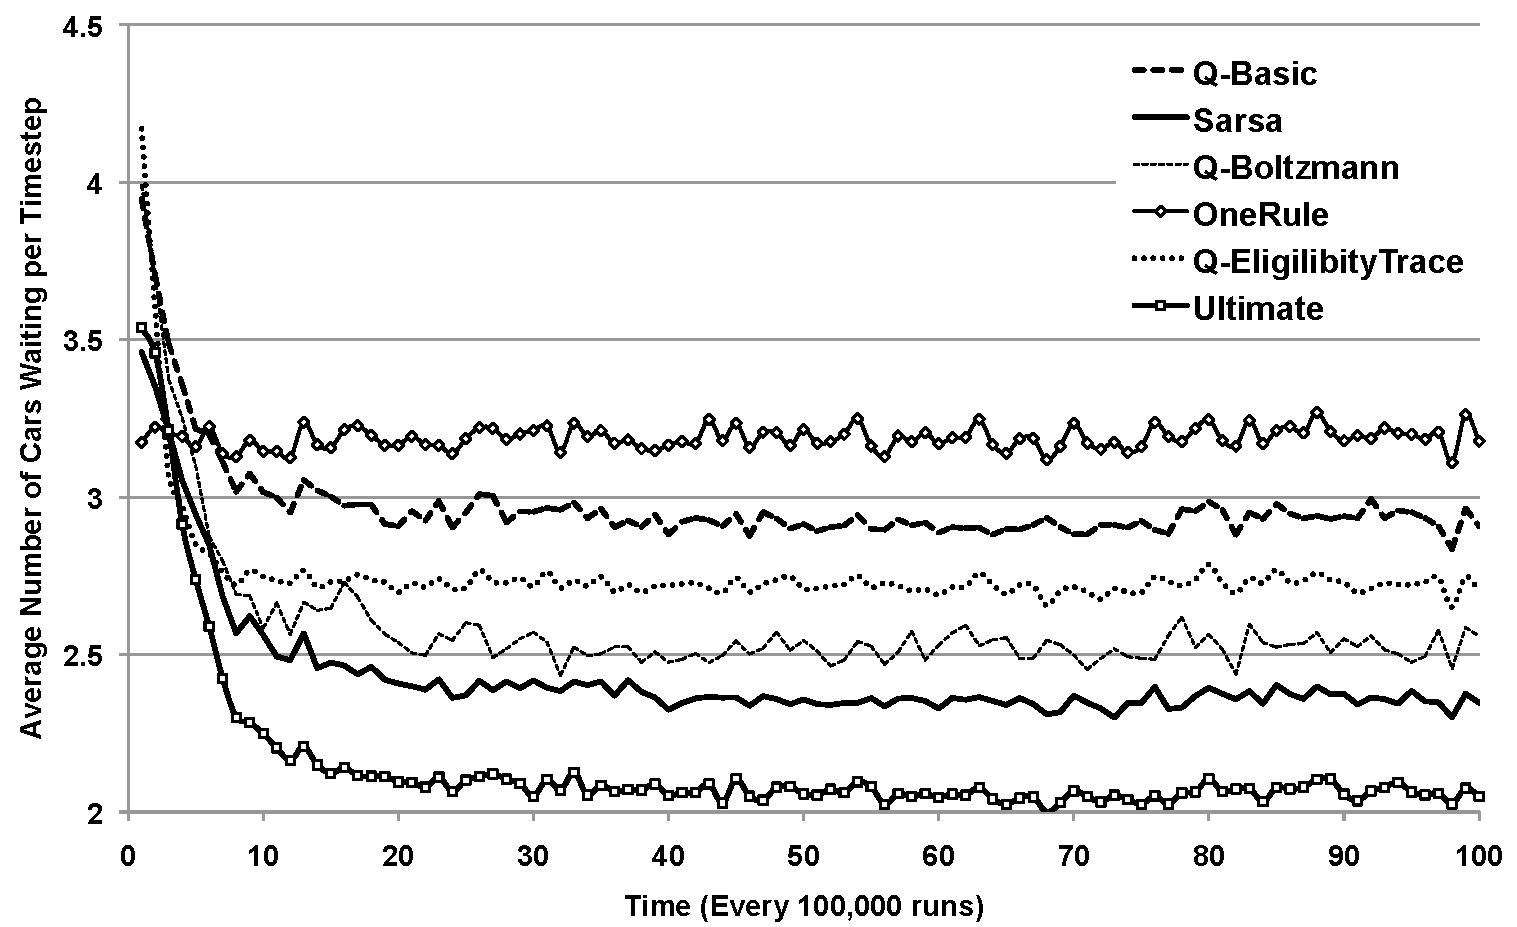
\includegraphics[width=0.45\textwidth]{algorithm}
\caption{Best Algorithm}\label{f:algorithm}
\end{figure}

\item[Fig.~\ref{f:algorithm}]
Discuss which algorithm is best.




\begin{figure}
\centering
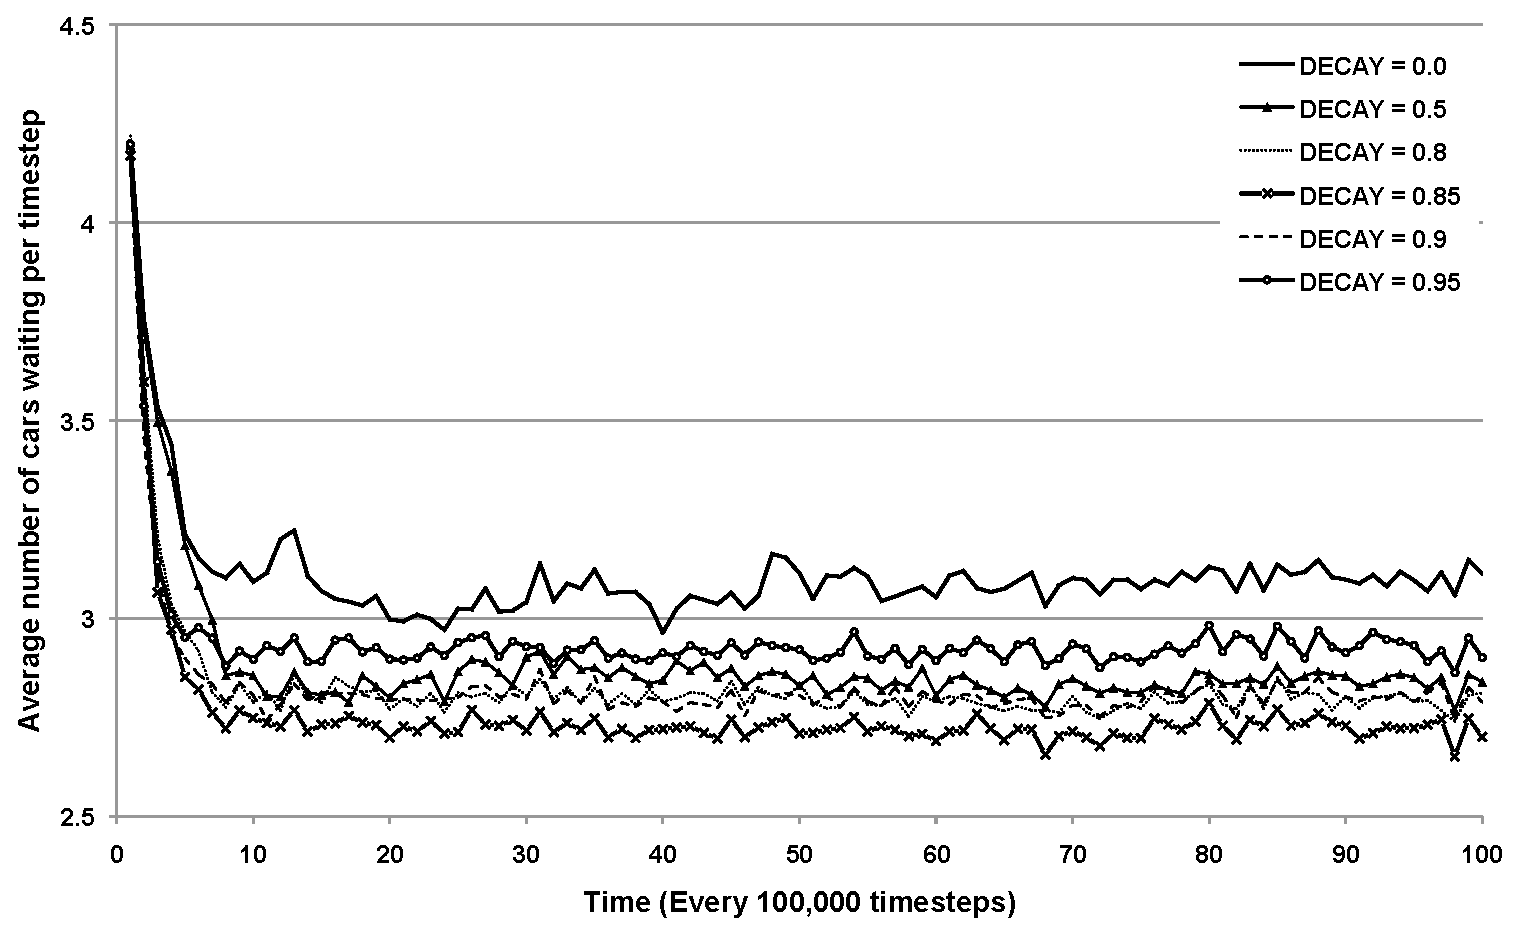
\includegraphics[width=0.45\textwidth]{eligibility}
\caption{Eligibility Trace}\label{f:eligibility}
\end{figure}

\item[Fig.~\ref{f:eligibility}]
Discuss eligibility trace.




\begin{figure}
\centering
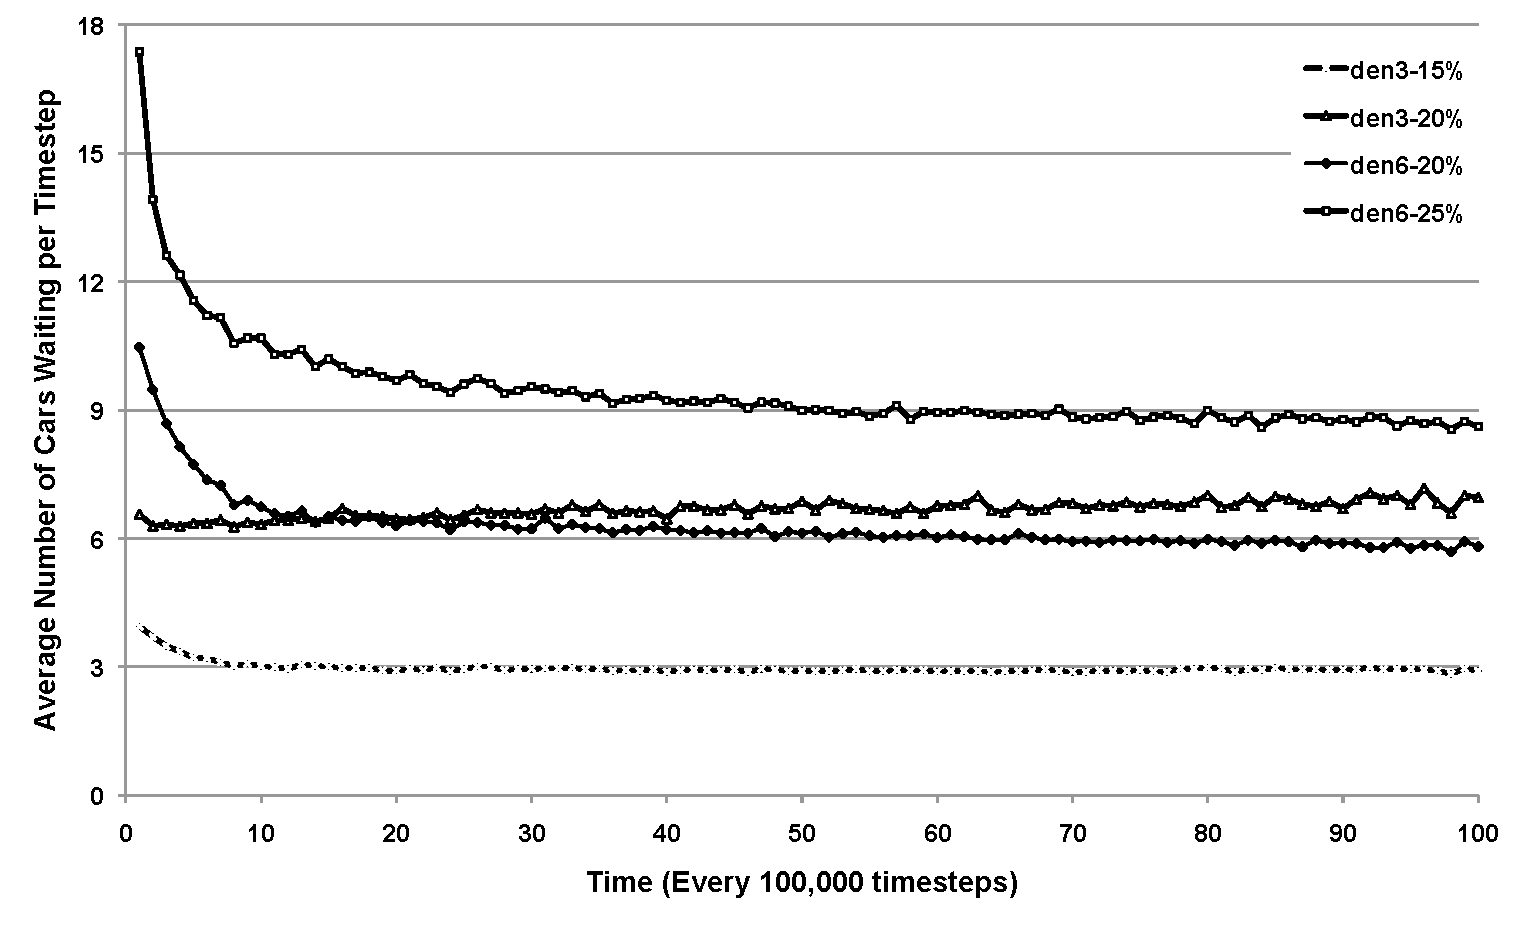
\includegraphics[width=0.45\textwidth]{intensity}
\caption{Varying Traffic Intensity}\label{f:intensity}
\end{figure}

\item[Fig.~\ref{f:intensity}]
Perhaps unsurprisingly, as the traffic intensity increases from 15\% to
25\%, we found more cars waiting for green light and the overall performance
drops. We have used the DensityState3 and DensityState6 at 20\% traffic
intensity and the performance is similar around 2,000,000 timesteps.
However, DensityState3 --- having a smaller state space --- starts to overfit
the traffic patterns whereas DensityState6 --- having a larger state space
--- continues to converge to optimal. Also, DensityState6 takes longer to
converge relative to DensityState3, most likely due to the larger state space.


\begin{figure}
\centering
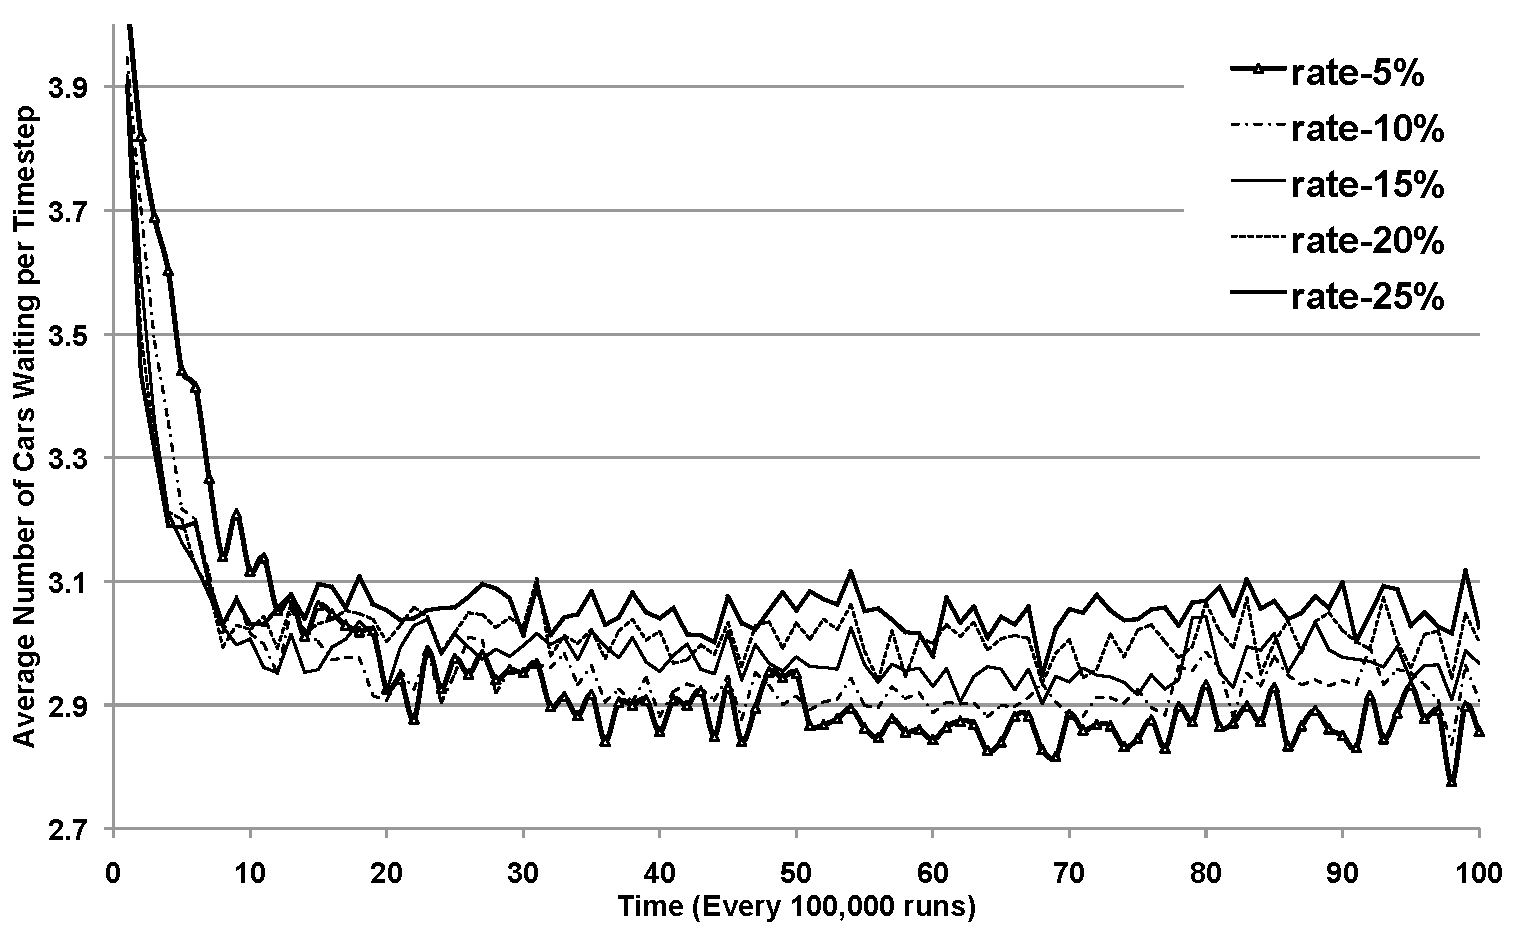
\includegraphics[width=0.45\textwidth]{learningRate}
\caption{Varying Learning Rate}\label{f:learningRate}
\end{figure}

\item[Fig.~\ref{f:learningRate}]
Discuss learning Rate.


\begin{figure}
\centering
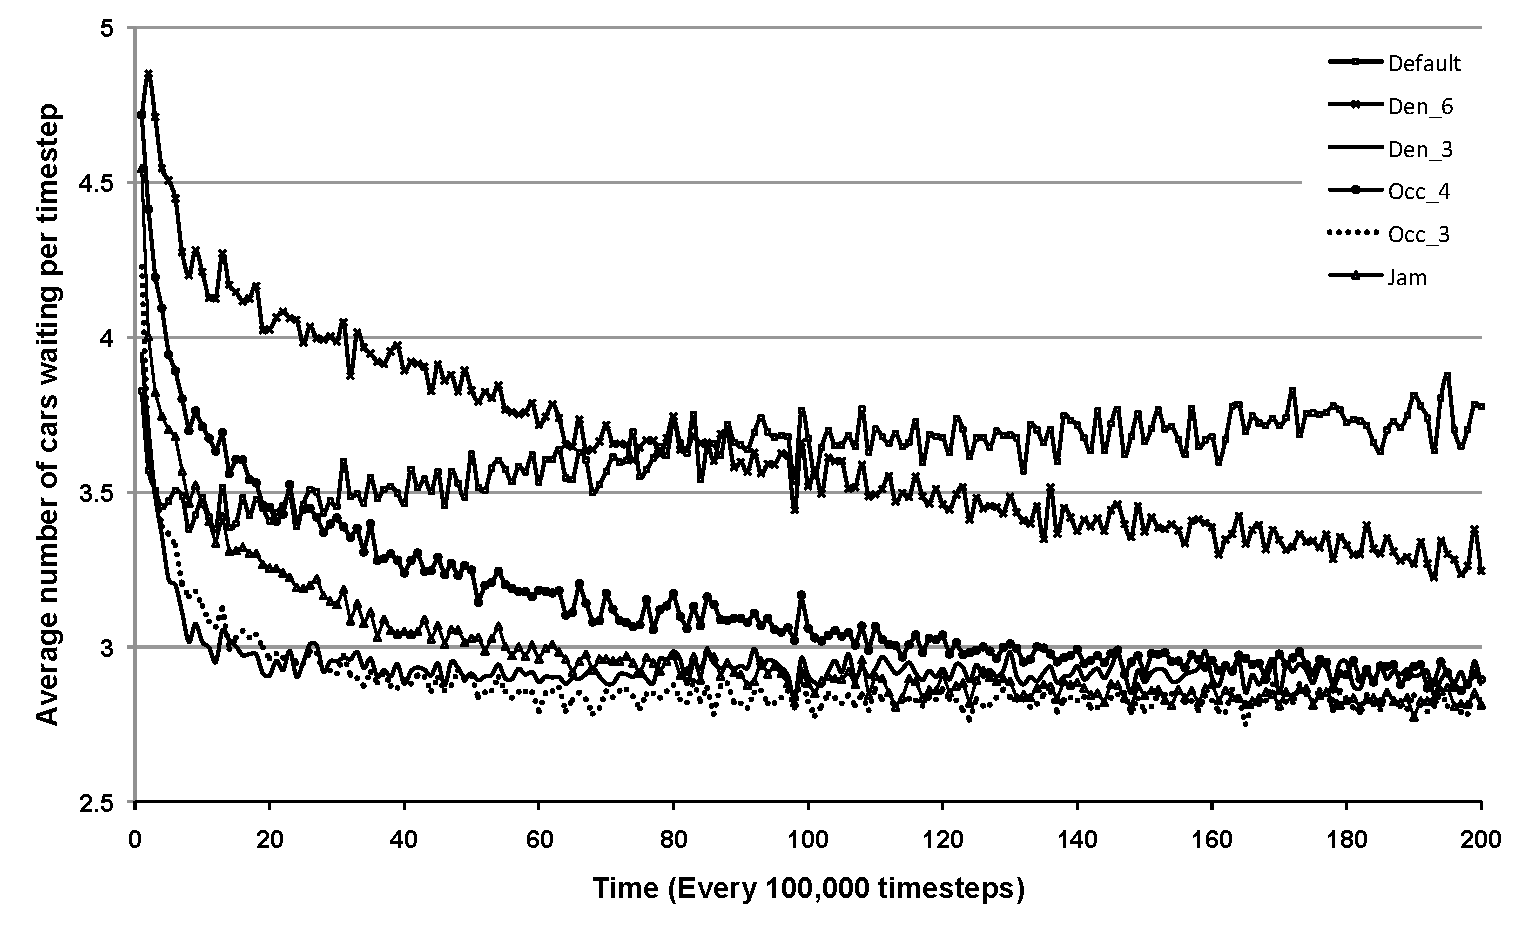
\includegraphics[width=0.45\textwidth]{states}
\caption{Varying State Representation}\label{f:states}
\end{figure}

\item[Fig.~\ref{f:states}]
Discuss learning Rate.



\begin{figure}
\centering
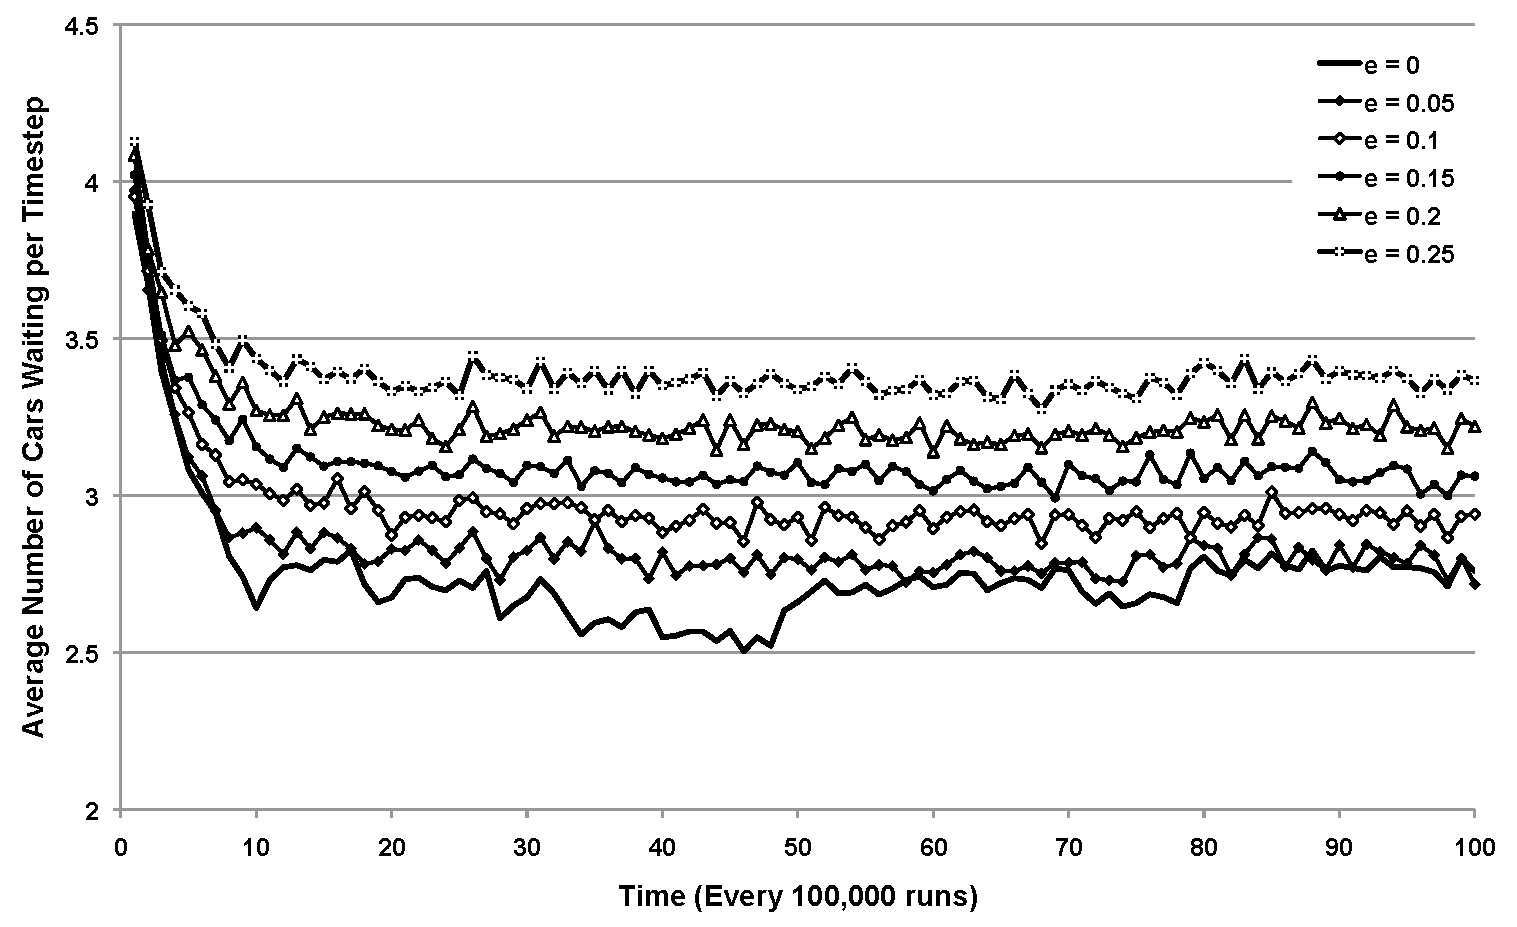
\includegraphics[width=0.45\textwidth]{epsilon}
\caption{Varying the $\epsilon $ value}\label{f:epsilon}
\end{figure}

\item[Fig.~\ref{f:epsilon}]
This experiment uses the benchmark settings except for the $\epsilon$
value (`e' in the figure) which is different in each run. For example $e = 0.25$ means
the QLearningBasic algorithm will explore 25\% of the time.
Note the $\epsilon$ is not discounted over time.
Better results are achieved with $\epsilon$ values near 0 but not 0,
suggesting that exploratory actions
that are not optimal are adding to the number of cars waiting; so
the less exploratory actions taken the better. However, some exploration
is required since $\epsilon =0$ shows that overfitting occurs after
about 4,600,000 timesteps. This overfitting is most likely due to
the algorithm finding the optimal action-value function for the traffic
pattern in the first 4.6 million timesteps, but the traffic patterns
in the following timesteps are different and the optimal policy is
no longer the most optimal.



\begin{figure}
\centering
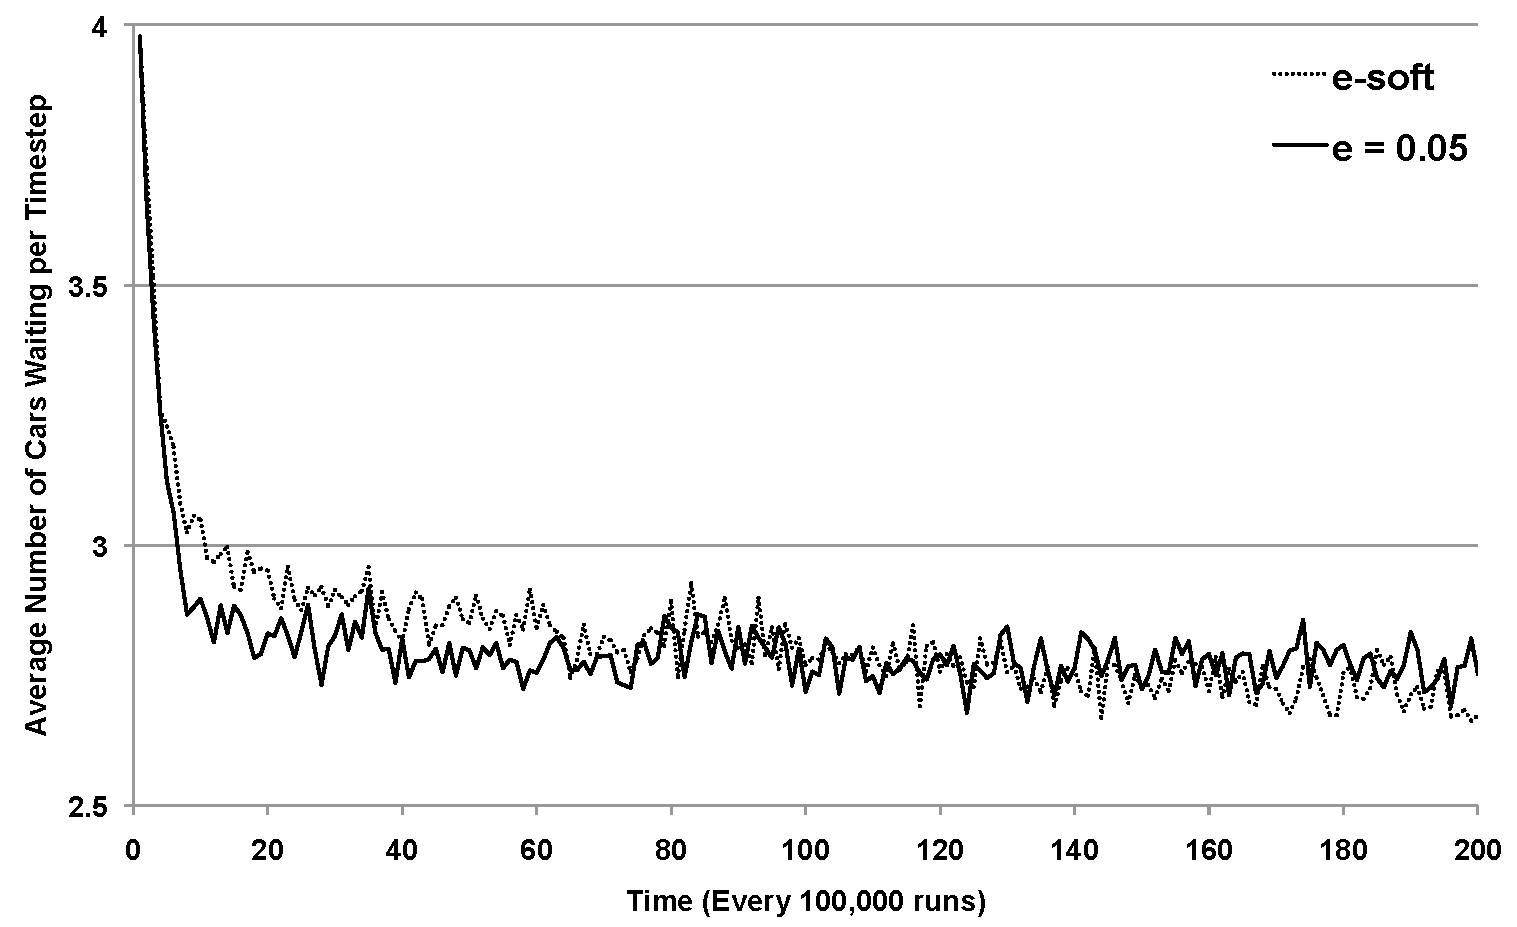
\includegraphics[width=0.45\textwidth]{e-soft}
\caption{Discounting $\epsilon$}\label{f:e-soft}
\end{figure}

\item[Fig.~\ref{f:e-soft}]
This figure shows the $\epsilon = 0.05$ result with a discounted
$\epsilon$ run. The discounted $\epsilon$ run uses the benchmark
settings (i.e. $\epsilon = 0.1$ initially) and discounting the
$\epsilon$ by 0.9999999 per timestep (that's seven 9s). The result shows
that a fixed $\epsilon$ stablises after about 4,300,000 timesteps
without further improvement; but the $\epsilon$-discounted algorithm
converges to the optimal as time progresses. This matches with what
\cite{Sutton_1998} says about Sarsa converges with probability
1 to an optimal policy only if the policy converges in the
limit to the greedy policy (i.e. $\epsilon$ tends to 0 in the limit);
although this is QLearningBasic algorithm and not Sarsa.




\begin{figure}
\centering
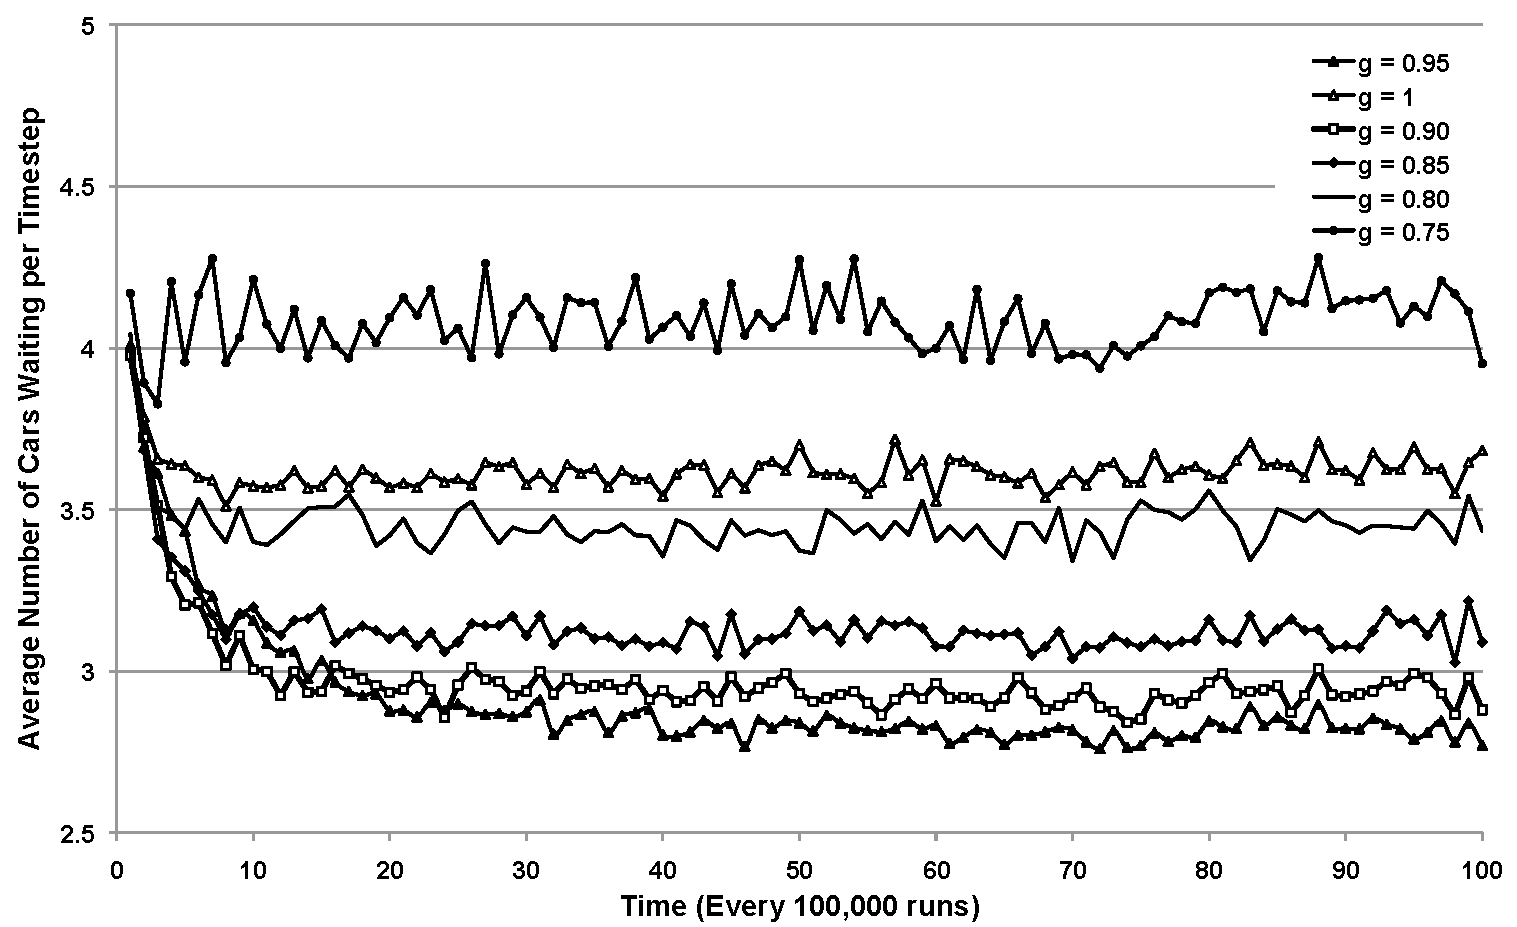
\includegraphics[width=0.45\textwidth]{discountFactor}
\caption{Varying the discount factor $\gamma$}\label{f:discountFactor}
\end{figure}

\item[Fig.~\ref{f:discountFactor}]
This experiment uses the benchmark settings except for the $\gamma$
discount factor (`g' in the figure) which is different in each run.
The results suggest the best discount factor to use is 0.95. As
$\gamma$ decreases from 0.95, the results gets progressively worse.
Values larger than 0.95 should also get worse, although we've only
done one run with $\gamma = 1$.

Why 0.95 is the best? I don't know.

\end{description}

\section {Conclusion}

Based on our results, the ``ultimate'' set-up is
(which algorithm?)
discount factor of 0.95
$\epsilon$-greedy with $\epsilon$ discounted over time at the rate of 0.99 99 99 9
OcupancyState3 representation
Learning rate of 0.05

This set-up will provide the best performance in the long-haul, which is
suitable for traffic light control since most traffic lights stay there
for a very long time. However, a much more cost effective
option is to build a roundabout, which saves electricity, saves maintenance
costs, saves having to write software to control traffic lights.


\bibliographystyle{abbrv}
\bibliography{autoscale_rl}  % sigproc.bib is the name of the Bibliography in this case

\balancecolumns
\end{document}
